In this chapter we present the SMT problem. Recall that our goal is to translate proofs of unsatisfiability of SMT queries into Lean proofs. Therefore, besides presenting formally the problem and explaining how it is solved, we focus on showing how proofs are represented in an SMT solver.

\subsection{Description of the Problem}

The Boolean Satisfiability Problem (SAT) consists of determining whether a formula in Propositional Logic, which contains free variables, can be evaluated to \textit{true} by finding a function that assigns a Boolean value to each variable.
We say that a formula is satisfiable if such a function exists, and unsatisfiable otherwise. In
this work, we will be focusing on the problem CNF-SAT, an equivalent version of SAT in
which the input formula always comes in Conjunctive Normal Form, that is, a conjunction
of disjunctions of literals. From now on, we will use SAT to refer to the CNF-SAT problem. Furthermore, we will write \textit{clause} to refer to each one of the disjunctions in some
input formula for SAT.\ We will also treat a clause as a set of its composing literals (a literal is either a variable or the negation of a variable) and use set operations over it. For instance, we will write $x \in C$ to state that the literal $x$ is present in clause $C$ and $C \setminus \{x\}$ to refer to the clause $C$ without the literal $x$.


Satisfiability Modulo Theories (SMT)~\cite[ch. 33]{handbook} is a generalization of SAT.\
There are two additions: first, the underlying logic framework is Equational First-Order
Logic instead of Propositional Logic. This means that the input formula
can contain quantifiers binding variables, unintepreted function symbols,
predicates asserting properties about variables and a special symbol ``$\simeq$'' that is used to assert equality between terms.
The second addition is the inclusion of a set of sorts, equipped with predefined
operations that allow the problem to refer to different domains.
For example, one instance of a problem in this extension can refer to variables
ranging over integers and contain assertions that compare the values of such variables.
This extension also permits the same instance of the problem to refer to multiple
distinct domains.
The logic framework that corresponds to Propositional Logic with these two additions is
known as Many-Sorted First Order Logic (MSFOL). The precise syntax and semantics of this
logic framework is given in detail for example in~\cite{many_sorted}. In
Section~\ref{sec:msfolHere} we give a brief overview of it.

\subsection{Many-Sorted First Order Logic}\label{sec:msfolHere}
\subsubsection{Syntax}

The syntax of MSFOL consists of three syntatic categories:

\begin{enumerate}
  \item \textbf{Sorts}. Symbols identifying the kinds of variables that are allowed. They are defined by the following grammar:
        \begin{center}
          $ \tau ::= \sigma \mid (\tau_{1}, \tau_{2}, \ldots, \tau_{n}) \rightarrow \tau$ % \mid (\tau_{1}, \tau_{2}, \ldots, \tau_{m})$
        \end{center}
        The first case represents an atomic sort drawn from a predefined set of sorts, which we will refer to as $\mathcal{S}_{S}$, and is required to have a cardinality that is at most countably infinite. The second case represents sorts of functions with arity $n$ whose return type is $\tau$. We will always assume that there is a special sort in $\mathcal{S}_{S}$ named $\textit{bool}$.
  \item \textbf{Terms}. Symbols representing sorted variables, constants or function applications. Function applications are only well formed when the sorts are respected. The symbols annotated on top of each term represent their sort, and they will be ommited when they can be inferred.
        \begin{center}
          $ t ::= x^{\tau} \mid f^{(\tau_{1}, \ldots, \tau_{n}) \rightarrow \tau}(t_{1}, \dots, t_{n}) $
        \end{center}
        where the return type of $f$ must be different than $bool$. Function symbols are also drawn from a predefined set, which we will refer to as $\mathcal{S}_{F}$, and it is also
        required to have a cardinality that is at most countably infinite. Constants are represented by nullary functions.
        Variables will also be drawn from a predefined set, which we will refer to as $\mathcal{S}_{X}$ and, again, impose the requirement of having a cardinality that is at most countably infinite.
  \item \textbf{Formulas}. Expressions built with logical connectives representing statements.
        \begin{center}
          $ \psi ::= p^{(\tau_{1}, \dots, \tau_{n}) \rightarrow bool}(t_{1}, \dots, t_{n}) \mid \psi_{1} \vee \psi_{2} \mid \forall x^{\tau}.\psi \mid \neg \psi \mid \psi_{1} \simeq \psi_{2}$
        \end{center}
        The first case is an \textit{atom}, that is, an application of a function whose return type is $bool$. This
        kind of function will be referred to as \textit{predicate}.
\end{enumerate}

We also define the following symbols:

\begin{center}
  $\exists x. \psi := \neg \forall x. \neg \psi$\\
  $\psi_{1} \wedge \psi_{2} := \neg (\neg \psi_{1} \vee \neg \psi_{2})$\\
  $\psi_{1} \rightarrow \psi_{2} := \neg \psi_{1} \vee \psi_{2}$\\
  $\psi_{1} \leftrightarrow \psi_{2} := \psi_{1} \rightarrow \psi_{2} \wedge \psi_{2} \rightarrow \psi_{1}$\\
  $\psi_{1} \not\simeq \psi_{2} := \neg (\psi_{1} \simeq \psi_{2})$
\end{center}

We define a \textit{signature} to be a triple of sets $\langle \mathcal{S}_{S}, \mathcal{S}_{F}, \mathcal{S}_{X} \rangle$ respecting the requirements defined above.

\subsubsection{Semantics}

Having established how terms in MSFOL are built, we have to define how they are evaluated, i.e.\ their meaning.
Given a signature $\Sigma = \langle \mathcal{S}_{S}, \mathcal{S}_{F}, \mathcal{S}_{X} \rangle$, a $\Sigma$\textit{-structure} is a function $\mathcal{I}$ that maps, for each sort symbol $s \in \mathcal{S}_{S}$, a corresponding set $\mathcal{I}(s)$, for each function symbol $f^{(\tau_{1}, \ldots, \tau_{n}) \rightarrow \tau} \in \mathcal{S}_{F}$, a function $\mathcal{I}(f)$ of type $\mathcal{I}(\tau_{1}) \times \cdots \times \mathcal{I}(\tau_{n}) \rightarrow \mathcal{I}(\tau)$ and for each variable $x \in \mathcal{S}_{X}$ of sort $s$, a value $\mathcal{I}(x) \in \mathcal{I}(s)$.
The $\textit{bool}$ sort will always be mapped to the usual set of Boolean values, and the set $\mathcal{S}_{F}$ will always contain two nullary functions, $\textit{true}$ and $\textit{false}$, which will be mapped to the usual true and false values, represented here respectively as $true^{I}$ and $false^{I}$.
A $\Sigma$\textit{-Theory} is a set of $\Sigma$-structures. Theories are used to refer to the multiple possible assignments
of values to variables in a formula.


Finally, we define the \textit{evaluation} of a given formula $\psi$ over a $\Sigma$-structure $\mathcal{I}$, denoted by $\llbracket \psi \rrbracket^{\mathcal{I}}$, in the following way:
\begin{align*}
  \llbracket x \rrbracket^{\mathcal{I}} &:= \mathcal{I}(x) \\
  \llbracket f(t_{1}, \ldots, t_{n}) \rrbracket^{\mathcal{I}} &:= D_{f}(\llbracket t_{1} \rrbracket^{\mathcal{I}}, \ldots, \llbracket t_{n} \rrbracket^{\mathcal{I}}) \\
  \llbracket \bot \rrbracket &:= false^{I} \\
  \llbracket t_{1} \simeq t_{2} \rrbracket^{\mathcal{I}} &:= \llbracket t_{1} \rrbracket^{\mathcal{I}} = \llbracket t_{2} \rrbracket^{\mathcal{I}} \\
  \llbracket \neg \psi \rrbracket^{\mathcal{I}} &:= \llbracket \psi \rrbracket^{\mathcal{I}} = false^{I} \\
  \llbracket \psi_{1} \vee \psi_{2} \rrbracket^{\mathcal{I}} &:= \llbracket \psi_{1} \rrbracket^{\mathcal{I}} = true^{I}\,\, or\,\, \llbracket \psi_{2} \rrbracket^{\mathcal{I}} = true^{I} \\
  \llbracket \forall x^{\tau} . \psi \rrbracket^{\mathcal{I}} &:= \llbracket \psi \rrbracket^{\mathcal{I}_{x \gets v}} = true^{I} \text{, for any } v \in \mathcal{I}(\tau)
\end{align*}
where $\mathcal{I}_{x \gets v}$ denotes the extension of the function $\mathcal{I}$ in which the variable $x$ is assigned the value $v$. We say that an structure $\mathcal{I}$ \textit{satisfies} a formula $\psi$ if and only if $\llbracket \psi \rrbracket^{\mathcal{I}} = true^{I}$. The structures that satisfy a formula $\psi$ are known as the \textit{models} for $\psi$. If there is at least
one model for a given formula $\psi$, it is said to be \textit{satisfiable}, otherwise it is \textit{unsatisfiable}.

\begin{example}[LIA]\label{ex:lia}
  Let $\mathcal{S}_{S} := \{Z\}$, $\mathcal{S}_{F} := \{add, sub, zero, succ, pred, lt\}$ and
  $S_{X} := \{x, y\}$. Examples of formulas that can be written using the signature composed by these sets include ``$lt(sub(x, y), succ(zero))$'' and ``$add(x, y) \simeq add(y, x)$''. For this particular signature, we can have many theories. For instance, if we fix $\mathcal{I}(Z) := \mathbb{Z}$ and the interpretation of each function symbol to its usual operation over integers, we can have an infinite set of structures, each one mapping $x$ and $y$ to a pair of integers. This set is a theory known as Linear Integer Arithmetic (LIA), which is able to express formulas involving
  linear arithmetic expressions over integers.
  On the other hand, if we let $\mathcal{I}(Z) := \mathbb{Z}_{13}$ and match each function symbol with the corresponding operation over integers modulo $13$, we have a theory representing formulas over integers modulo $13$.
\end{example}

\subsection{SMT Solvers}

An SMT solver is a piece of software whose main goal is to solve the SMT problem, that is, determining whether a given formula expressed in MSFOL is satisfiable or not.
%
This problem is undecidable in its most general form. However, some variants of it which restrict the input formula
to be expressed over certain theories (such as LIA) are known to be decidable.
%
Thus, in order to achieve their goal, SMT solvers utilize a combination of
heuristics (for managing undecidable theories) along with decision procedures (for those theories known to be decidable).
%
In this section we present the methods employed by these systems that are more relevant to the present work.

\subsubsection{Davis–Putnam–Logemann–Loveland Algorithm (DPLL)}

First, let’s explore how SAT is solved. Although MSFOL is not decidable, Propositional Logic (PL) is, therefore, it is possible to design a decision procedure for SAT.\@
%
Indeed, one simple way to check whether a formula in Propositional Logic (PL) with $n$ variables is satisfiable or not, is to
test whether each one of the $2^{n}$ functions that assign truth values to those variables satisfies the formula.

A more efficient alternative of a decision procedure for PL is the DPLL algorithm~\cite{dpll}. DPLL is based on the \textit{Resolution} theorem:

\begin{theorem}[Resolution]\label{res_theorem}
Let $x$ be a literal. Let $C_{1}$ and $C_{2}$ be two clauses such that $x \in C_{1}$ and $\neg x \in C_{2}$. Then $C_{1} \wedge C_{2} \rightarrow (C_{1} \setminus \{x\}) \vee (C_{2} \setminus \{\neg x\})$.
\end{theorem}
More specifically, it is based on \textit{Unit Resolution} (UR), that is, a more restricted version of resolution in which $C_{1} = \{x\}$ or $C_{2} = \{\neg x\}$. Notice that the clause that is inferred from the unit resolution theorem is equal to one of the clauses in the premisses, with one less literal. The general idea of the DPLL algorithm is to explore this fact to generate smaller clauses, while this is possible. Once all possible unit resolutions are performed, the algorithm makes a decision, assigning a boolean value to a variable. This action can potentially create more clauses suitable for unit resolution, which will be then explored. If this decision does not lead to the conclusion that the original formula is satisfiable, the procedure backtracks and assigns the other boolean value to the variable. If this decision also does not lead to a positive conclusion, then the original formula is unsatisfiable.

\begin{figure}[t]
% \textbf{Input:} $\psi$, a PL formula\\
% \textbf{Output:} \textit{true} or \textit{false}, depending whether $\psi$ is satisfiable
\begin{algorithmic}[1]
\Function{SolvePL}{$\psi$}
\If{$\exists C \in \psi .\, C = \{\} \vee C = \{\bot\}$}
  \State \Return~\textit{false}
\EndIf
\If{$\forall C \in \psi .\, \top \in C$}
  \State \Return~\textit{true}
\EndIf
\If{$\exists x \in \mathit{Vars}(\psi) \,$ such that $x$ is a target for UR}
  \State $\langle C_{1}, C_{2} \rangle \gets$ \Call{findClauses}{$x$, $\psi$} \Comment{Suitable for applying UR with $x$}
  \State~\Return~\Call{SolvePL}{$\psi \wedge (C_{1} \setminus \{x\} \vee C_{2} \setminus \{\neg x\})$}
\EndIf
\State Let $x$ be an unassinged variable in $\psi$
\State \Return~\Call{SolvePL}{$\psi_{\{x \gets \top\}}$} $\vee$ \Call{SolvePL}{$\psi_{\{x \gets \bot\}}$}
\EndFunction
\end{algorithmic}
\caption{DPLL Algorithm}~\label{dpllAlgo}
\end{figure}

Figure~\ref{dpllAlgo} shows an algorithm for DPLL.\ The procedure \textit{SolvePL} works as follows: first, in lines 2 to 7, it checks if the formula can be evaluated to \textit{true} or \textit{false}. In case it is not possible, the procedure finds as many variables in which it can apply Unit Resolution as possible, using the routine \textit{findClauses}, and invokes itself recursively with each new application found, as shown in lines 8 to 10. By the resolution theorem, the formula that will be used as a parameter in the recursive call is satisfiable if and only if the one that was received as input is also satisfiable, therefore, this step is sound. Once there are no more possibilities, it chooses an arbitrary variable and makes two recursive calls in line 13: one assigning this variable to \textit{true} and the other one to \textit{false}. Since these are the only two possibilities for that variable, the input formula is satisfiable if and only if one of the recursive calls returned \textit{true}. The algorithm uses this information to correctly return the disjunction between the two return values.

For instance, let's run the algorithm with $\psi := \{\neg x, x \vee y, x \vee \neg y\}$. Neither of the
checks of lines 2 and 5 will succed with this formula. The check on line 8 will, since we can apply unit resolution on the first and second clauses, eliminating the variable $x$. This will produce the new clause $y$.
Following the algorithm, we apply the function $solvePL$ using $\{\neg x, x \vee y, x \vee \neg y, y\}$ as the
argument. The checks on lines 2 and 5 will fail again. We can apply unit resolution again using the clauses $\neg x$ and $x \vee \neg y$, eliminating $x$. This will produce the clause $\neg y$. We add it to the input formula
and run the function again. Once more, the checks on lines 2 and 5 will fail, and we will be able to apply
unit resolution to the clauses $y$ and $\neg y$, resulting in the empty clause. Now, when we invoke the function
recursively again, the check on line 2 will succed, and it will correctly return $false$.

The actual algorithm used by most SMT solvers to solve SAT is a refinement over DPLL, called Conflict Driven Clause Learning (CDCL)~\cite{cdcl}. Its main idea is to modify the DPLL algorithm so that, when it finds a conflict (an empty clause or a clause that only contains false variables), analyze the reason for this conflict, allowing it to derive new clauses and to backtrack many decisions of values of variables at once.
The DPLL algorithm also obtain information from conflict, but it cannot backtrack many decisions at once.
The new clauses derived from the analysis performed by CDCL can also be inferred via resolution.
Since our main concern in this work is on proofs, and, as we will show, proofs for unsatisfiability
of Boolean formulas are given in terms of resolution inferences, this refinement is not relevant
for our work and we will not present it in detail here.

\subsubsection{Proof Certificates for Boolean formulas}

In order to convince the ITP that the result found by the SMT solver is correct, we need evidence provided by the
ATP.
%
We will refer to such evidence as proof certificate.
%
The main feature of a good certificate is being easy to check.
%
In particular, it is desirable that it is easier to check a certificate then to solve the original problem.
%
The theories that are of our interest in this project have already been instrumented in cvc5 enabling the solver to produce proof certificates for them~\cite{Barbosa2022}.

If the SMT solver found out that a given formula is satisfiable, then it can always provide the model for that formula as a certificate. If the input formula is unsatisfiable, then this option is not available, so it is more challenging to provide such certificate. In this work we will focus on proof certificates for the unsatisfiability of formulas.

The main proof certificate produced by SMT solvers for the unsatisfability of instances of the SAT problem is
a \textit{resolution tree}. A resolution tree is a binary tree in which each leaf correspond to a clause from the SAT instance, each internal node correspond to the clause resulting of applying the Theorem~\ref{res_theorem} on its two children and the root corresponds to the empty clause.

For instance, for the example we provided for the DPLL algorithm, the resolution tree that corresponds to that
particular execution of the algorithm is the following:
\[
  \infer{\bot}{\infer{y}{\neg x & x \vee y} & \infer{\neg y}{\neg x & x \vee \neg y}}
\]

% For instance, let's run the algorithm with $\psi := \{x \vee y, x \vee \neg y \vee z, \neg x \vee z, \neg z\}$. Neither
% of the checks of lines 2 and 5 will succed with this formula. The check on line 8 will succed, since we can apply unit resolution on the second and fourth clauses, eliminating the variable $z$. This will produce the new clause $x \vee \neg y$. Following the algorithm, we apply the function recursively with $\psi$ extended with this new clause. The checks on lines 2 and 5 fail again. We can apply unit resolution again using the clauses $\neg x \vee z$ and $\neg z$, eliminating $z$. This will produce the clause $\neg x$. We add it to the input formula and run the algorithm again. Once more, the checks on lines 2 and 5 fail, and we can apply resolution with the clauses
% $x \vee y$ and $\neg x$, yielding $y$. We run the algorithm once more, with the singleton $\{y\}$ added to the

\subsubsection{CDCL(T)}

Assuming that we have a decision procedure for a given theory (or a combination of them), we can use it to extend the CDCL algorithm for checking the satisfiability of MSFOL formulas involving that theory. In this section we will study the CDCL(T)~\cite{cdcl_t} framework, a method for doing this extension over CDCL.\

\begin{figure}[t]
% \textbf{Input:} $\psi$, a formula in MSFOL over a theory  $\mathcal{T}$ \\
% \textbf{Output:} \textit{true} or \textit{false}, depending whether $\psi$ is satisfiable
\begin{algorithmic}[1]
\Function{SolveMSFOL}{$\psi$}
\State $\psi_{CNF} \gets \Call{ConvertCNF}{\psi}$
\State $\psi_{PL} \gets \Call{Convert}{\psi_{CNF}}$ \Comment{Get PL formula from MSFOL formula}
\If{$\Call{CDCL}{\psi_{PL}}$}
  \State $\mathcal{I} \gets \Call{GetModel}{\psi_{PL}}$
  \If{$\Call{TheorySolver}{\mathcal{I}, \psi}$} \Comment{Check if $\mathcal{I}$ is compatible with $\psi$}
    \State \Return \textit{true}
  \EndIf
  \State $L \gets \Call{GetConflictingLemma}{\mathcal{I}, \psi}$
  \State \Return $\Call{SolveMSFOL}{\psi \wedge L}$
\EndIf
\State \Return \textit{false}
\EndFunction
\end{algorithmic}
\caption{CDCL(T) Algorithm}~\label{cdclTAlgo}
\end{figure}

Consider a formula $\psi$ over a theory $\mathcal{T}$ in MSFOL.\ Let's assume we have a solver for this theory (that is, a method for deciding whether a given conjunctive set of propositions in $\mathcal{T}$ is consistent or not). We do not need the theory solver to handle disjunctions between propositions since the CDCL(T) algorithm will leverage a SAT solver to handle this part of the analysis. The first step of the algorithm is to obtain a formula $\psi_{CNF}$ equisatisfiable with $\psi$\footnote{i.e. $\psi_{CNF}$ is satisfiable if and only if $\psi$ is satisfiable} that is in conjunctive normal form. Then, it will create a PL formula $\psi_{PL}$ from $\psi_{CNF}$ by substituting each atom built from a predicate of $\mathcal{T}$ in it for a fresh Boolean variable. We can then use the previously described CDCL algorithm to determine whether $\psi_{PL}$ is satisfiable. For instance, consider $\psi$ to be the formula $x > 3 \wedge x < -2$. From it, we would generate the PL formula $p \wedge q$, where $p$ represents $x > 3$ and $q$ represents $x < -2$. If $\psi_{PL}$ is unsatisfiable, then $\psi$ is also unsatisfiable. If this was not the case, it would be possible for $\psi_{PL}$ to be unsatisfiable and $\psi$ be satisfiable. This means that there would exist a model for $\psi$. From this model, we would be able to derive truth values for the variables in $\psi_{PL}$ that should satisfy the formula, but this is an absurd since $\psi_{PL}$ is unsatisfiable.
If $\psi_{PL}$ is satisfiable, we can find a model $\mathcal{I}$ for $\psi_{PL}$. Although $\mathcal{I}$ satisfies $\psi_{PL}$, it is possible that it is contradictory in the context of the theory $\mathcal{T}$. In our previous example,
the only possible model for $\psi_{PL}$ is the one that assigns $p$ and $q$ to $true^{I}$, but this is not valid when we translate back to $\psi$, as $x$ cannot be both greater than $3$ and smaller then $-2$.
 If this happens, we rely on the theory solver to provide a new lemma from $\mathcal{T}$ that shows why the previous assignment was invalid. In this case, it would provide the lemma $\neg (x > 3 \wedge x < -2)$. Note that we are assuming that our theory solver has the capability of producing such a conflicting lemma for a particular model.


Figure~\ref{cdclTAlgo} shows an implementation of CDCL(T). The procedure \textit{SolveMSFOL} works as follows: first, in line 2, we convert the formula to CNF. Then, in line 3 perform the conversion that we just described, in order to obtain a PL formula. Next, in line 3, we run the procedure \textit{CDCL} to determine if $\psi_{PL}$ is satisfiable. In case it is not, we just return \textit{false} in line 12. Otherwise, there exists an model $\mathcal{I}$ that satisfies $\psi_{PL}$. This model is obtained in line 5 and we proceed to check if the theory solver accepts it for $\psi$ in line 6. If it does accept, the formula is definitely satisfiable and we can return \textit{true}, as done in line 7. Otherwise, the conflicting lemma for the given model is generated in line 9. We then repeat this process in line 10, adding the conflicting lemma to $\psi$.

\subsubsection{Equality and Uninterpreted Functions}\label{sec:euf}

In this work, we will be interested in two theories and their respective solvers. The first one is Equality and Uninterpreted Functions.

Consider the following problem: given a set of variables and uninterpreted functions and a set of equalities built from variables and functions applied to those variables, decide whether a given equality is a consequence of the conjunction of the ones in the set. For instance, let $a$, $b$, $c$ and $d$ be variables and $f$ a function of arity $1$. Assume that all variables belong to an artificial sort $U$, and all functions both take arguments and return values of this sort. The set $S := \{b \simeq c, f(b) \simeq c, f(c) \simeq a\}$ has as one consequence the equality $a \simeq b$.

Given a set $S$ of equalities between terms, the set of all equalities (only involving those terms) that can be
derived from the elements of $S$ is known as the \textit{congruence closure} of $S$.
%
Deciding whether a given equality is in the congruence closure for a given set is an old problem, which was shown to be decidable by Ackermann in 1954~\cite{ack_cong}. It is also is used as the basis for the theory of Equality and Uninterpreted Functions (EUF) in SMT, as we will see later.

This theory is used to express satisfiability problems involving equalities
and inequalities of variables and function applications. Since the language of
MSFOL already has a built-in equality operator, we do not need to fix the meaning
of any operator in this theory. Its semantics are the same of Equational First-Order
Logic without any addition. For this reason, this theory is also known as the
``empty theory''.

We now give a brief overview on the standard algorithm for finding the congruence closure of a given set of equalities. A more detailed explanation can be found at~\cite{orig_cong_clos}. This solution is based on the concept of congrunce.
Congruence is a property that all function applications enjoy:
if $f$ is a function of arity $n$ and ${(a_{k})}_{k = 1}^{n}$ and ${(b_{k})}_{k = 1}^{n}$ are two sequences of terms such that $a_{i} \simeq b_{i}$ for all $i$, then
$f(a_{1}, \ldots, a_{n}) \simeq f(b_{1}, \ldots, b_{n})$.

% \begin{theorem}[Congruence]\label{cong_theorem}
% Let $f$ be a function of arity $n$ and ${(a_{k})}_{k = 1}^{n}$ and ${(b_{k})}_{k = 1}^{n}$ be two sequences of terms. $\bigwedge_{i = 1}^{n} a_{i} = b_{i} \rightarrow f(a_{1}, \ldots, a_{n}) = f(b_{1}, \ldots, b_{n})$.
% \end{theorem}

Let $S$ be the set of equalities that are assumed and $e$ be the one that we want to decide whether is a consequence of $S$. Let $T$ be the set of all terms that appear in $S \cup \{e\}$ including all function parameters. Let's build a graph $G$ in which for all $t \in T$ we will have a vertex $v$ in $G$ that represents that term. For the vertex $v$, we will assign a label with the name of the term it represents. Moreover, if $t$ is a function application we will add directed edges from $t$ to each vertex that represents a term that is an argument to $t$. Also, we will keep an order over the children for each vertex, according to the order in which the parameters are applied. For instance, let $S := \{f(a, b) \simeq a\}$ and $e := f(f(a, b), b) \simeq a$. Then we would build $G$ as follows:

\renewcommand{\algorithmicforall}{\textbf{for each}}
\MakeRobust{\Call}

\begin{figure}[t]
\begin{algorithmic}[1]
  \Procedure{MergeCong}{$v_{1}$, $v_{2}$}
  \If{$\neg$ \Call{SameClasses}{$v_{1}$, $v_{2}$}}
    \State Let $v_{1}^{*}$ and $v_{2}^{*}$ be the equivalence classes of $v_{1}$ and $v_{2}$.
    \State Let $P_{v_{1}^{*}}$ be the set of all predecessors of all vertices in $v_{1}^{*}$
    \State Let $P_{v_{2}^{*}}$ be the set of all predecessors of all vertices in $v_{2}^{*}$
    \State\Call{Merge}{$v_{1}$, $v_{2}$}
    \ForAll{$u_{1} \in P_{v_{1}^{*}}$ and $u_{2} \in P_{v_{2}^{*}}$}
      \If{\Call{IsCongruent}{$u_{1}$, $u_{2}$}}
        \State \Call{MergeCong}{$u_{1}$, $u_{2}$}
      \EndIf
    \EndFor
  \EndIf
  \EndProcedure
\end{algorithmic}
\caption{Merge with Congruence}~\label{merge_cong}
\end{figure}

\begin{figure}[h]
\centering
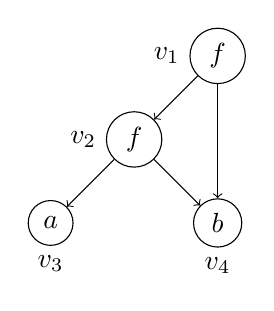
\begin{tikzpicture}[node distance={15mm}, main/.style = {draw, circle}]
\node[main, label=left:$v_{1}$] (1) {$f$};
\node[main, label=left:$v_{2}$] (2) [below left of=1] {$f$};
\node[main, label=below:$v_{3}$] (3) [below left of=2] {$a$};
\node[main, label=below:$v_{4}$] (4) [below right of=2] {$b$};
\draw[->] (1) -- (2);
\draw[->] (2) -- (3);
\draw[->] (2) -- (4);
\draw[->] (1) -- (4);
\end{tikzpicture}
\end{figure}

For a vertex $v$, we will denote by $\lambda(v)$ its label, $\delta(v)$ its outdegree and $Child(v, i)$ its $i$-th child.
Next, we will keep a data structure that is capable of representing a set of disjoint sets of vertices. Each one of these disjoint sets represents a class in an equivalence relation, where every vertex in the same class is known to be equal. This data structure must also be able to check whether two vertices are on the same class and to join two classes. An example of structure with such capabilities that is efficient and easy to implement is the Union-Find~\cite{union_find}.

Initially, each term is only equal to itself. Then, for each equality $t_{1} \simeq t_{2}$ in $S$ we will use the procedure \textit{MergeCong} presented in Figure~\ref{merge_cong} to merge the vertices $v_{1}$ and $v_{2}$ that correspond to $t_{1}$ and $t_{2}$.
Notice that, when we process an equality $t_{1} \simeq t_{2}$, we also have to propagate this information to any other terms that are using $t_{1}$ and $t_{2}$ as parameters (e.g.~if we have $f(t_{1})$ and $f(t_{2})$ as terms, we must also merge their classes). That's why we recursively call \textit{MergeCong} on line 11.
This method has an auxiliary procedure for checking whether two vertices are congruent given the current state. Figure~\ref{cong_cond} shows an implementation of this method, which essentially just checks the premise of the congruence property.

\begin{figure}[t]
\begin{algorithmic}[1]
  \Function{IsCongruent}{$v_{1}$, $v_{2}$}
  \If{$\lambda(v_{1}) \neq \lambda(v_{2})$ or $\delta(v_{1}) \neq \delta(v_{2})$}
    \State\Return~$false$
  \EndIf
  \For{$i = 1$ to $\delta(v_{1})$}
  \If{$\neg$ \Call{SameClasses}{\Call{Child}{$v_{1}$, $i$}, \Call{Child}{$v_{2}$, $i$}}}
      \State\Return $false$
    \EndIf
  \EndFor
  \State\Return $true$
  \EndFunction
\end{algorithmic}
\caption{Check Congruence Condition}~\label{cong_cond}
\end{figure}


Once this process is done, we can check whether any pair of terms $t_{1}$ and $t_{2}$ is currently equal to each other by checking whether their corresponding vertices $v_{1}$ and $v_{2}$ are on the same equivalence class (i.e.\ checking whether $Find(v_{1}) = Find(v_{2})$). Therefore, we can use this fact to solve our original problem of checking if the equality $e$ follows from the conjunction of the equalities in $S$.

% you must say that the graph is build using the inequalities too
Given a conjunctive set of propositions in the theory of Equality and Uninterpreted Functions, we can check
its satisfiability in the following manner: we build the graph mentioned earlier using
all terms appearing in the set (both in equalities and in inequalities). Then, for
each equality $t_{1} \simeq t_{2}$ we call the procedure $MergeCong$ to merge the vertices corresponding to $v_{1}$ and $v_{2}$.
Lastly, for each inequality $t_{1} \not\simeq t_{2}$, we check if the vertices corresponding to $t_{1}$ and $t_{2}$ are on the same equivalence class. If this is the case for any inequality, the set is unsatisfiable. Otherwise, it is satisfiable.

\subsubsection{Proof Certificates for EUF}

The algorithm we presented for computing the satisfiability of a conjunctive set of
atoms from EUF can be instrumented in a way that, if it derives that a formula is
unsatisfiable, it produce a proof tree, similar to the resolution tree, that
certificates this result.
The only difference between this proof tree and the resolution tree is that, instead of using the resolution theorem to infer new propositions, the proof tree will use the axioms that equality satisfies (reflexivity, symmetry and transitivity), as well as the congruence property. For instance, consider the following set of propositions: $\{a \simeq f(f(a)), a \simeq f(f(f(a))), f(a) \not\simeq a\}$. One possible proof tree that certificates its unsatisfiability is the following:

\[
  \infer[]{\bot}{\infer[trans]{f(a) \simeq a}{\infer[cong]{f(a) \simeq f(f(f(a)))}{a \simeq f(f(a))} & \infer[symm]{f(f(f(a))) \simeq a}{a \simeq f(f(f(a)))}} & f(a) \not\simeq a}
\]

\subsubsection{Linear Arithmetic}

The second theory that we will be interested in this work is the theory of Linear Arithmetic. A term in this theory is an expression of the form:
\begin{center}
  $\mathlarger{\sum}_{i = 1}^{n} a_{i} x_{i} \bowtie b$
\end{center}

Where each $a_{i}$ and $b$ are constants ranging over the real numbers, each $x_{i}$ is a variable and $\bowtie$ is one of $\le$, $<$ or $\simeq$ (we model $\ge$ and $>$ as the negation of $<$ and $\le$). If we allow variables to range only over integers (represented by the \textit{Int} sort), we have the Linear Integer Arithmetic theory, which was described in terms of MSFOL in Example~\ref{ex:lia}. If variables can range over the real numbers (represented by the \textit{Real} sort), the corresponding theory is known as Linear Real Arithmetic (LRA), which can be described using MSFOL a similar way.

We will now review the method presented in~\cite{simplex_dpllt} for checking whether a given set of atoms from LRA is satisfiable. This is the method generally employed by SMT solvers (in particular, by cvc5) to solve problems in this theory. It is broadly employed due to its amenability to run incrementally, an important feature in the CDCL(T) framework. The paper also presents an extension of this method for LIA, which we will not show here for brevity.

The first step is to, for each atom $t_{i} \bowtie b_{i} \in \phi$ in which $t_{i}$ is a sum of at least two variables, create a fresh variable $s_{i}$. Then, we will define two new sets of atoms: $\phi_{A}$, such that its atoms are all of the form $s_{i} \simeq t_{i}$, that is, they state the equality between the new variables and the corresponding terms, and $\phi'$, that has all the atoms in $\phi$ but with each term $t_{i}$ substituted by the corresponding $s_{i}$. For instance, let the set of atoms be
$\phi := \{x - y \ge 3, x - 2y < 6, x - y \le 10, x \ge 5\}$.  From this, we would define $\phi_{A} := \{s_{1} = x - y, s_{2} = x - 2y\}$ and $\phi' := \{s_{1} \ge 3, s_{2} < 6, s_{1} \le 10, x \ge 5\}$. Note that $\phi$ and $\phi_{A} \wedge \phi'$ are equisatisfiable, since we can rewrite the equations from $\phi_{A}$ in $\phi'$ to obtain the atoms in $\phi$.

Next we will represent the restrictions in $\phi_{A}$ as $Ax = 0$, where $A$ is a matrix and $x$ is a vector with all the variables in the problem (including the ones we added). We build the $i$-th row in $A$ with the coefficients for each variable in the equation for $s_{i}$ in $\phi_{A}$. We will refer to the entry in the $i$-th row and $j$-th column of $A$ as $a_{ij}$. If the original problem had $n$ variables and we added $m$ fresh ones, the matrix $A$ will have $m$ rows and $m + n$ columns. In our example, we would have the following:

\begin{center}
$
A :=
\begin{bmatrix}
  1 & -1 & -1 & 0 \\
  1 & -2 & 0 & -1
\end{bmatrix}
x :=
\begin{bmatrix}
  x & y & s_{1} & s_{2}
\end{bmatrix}^{T}
$
\end{center}

\begin{figure}[t]
\begin{algorithmic}[1]
  \Procedure{Update}{$v_{i}$, $val$}
  \For{$v_{j} \in \mathcal{B}$}
    \State $\beta(v_{j}) \gets \beta(v_{j}) + a_{ji}(v - \beta(v_{i}))$
  \EndFor
    \State $\beta(v_{i}) \gets val$
  \EndProcedure
\end{algorithmic}
\caption{Change value of non-basic variable and update all basic variables}
\end{figure}

Now, our problem is reduced to finding a vector $x$ that satisfies $Ax = 0$ and respects all restrictions in $\phi'$, which are all of the form $v_{i} \bowtie b_{i}$, where $v_{i}$ is one of the variables and $b_{i}$ is a constant. We will assume that there is no strict inequalities in $\phi'$ for brevity. For an extension of the method presented here for strict inequalities, consult~\cite{simplex_dpllt}. Notice that in this case we can represent the restrictions in $\phi'$ as two sequences of coefficients $l_{i}$ and $r_{i}$, representing a sequence of restrictions of the form $l_{i} \le v_{i} \le r_{i}$, as long as we allow $l_{i}$ to be $-\infty$ in case there is no lower restriction on $v_{i}$ and $r_{i}$ to be $+\infty$ in case there is no upper restriction on $v_{i}$.

We will solve this problem by processing each restriction in $\phi'$ incrementally. The algorithm maintains a state that includes the coefficients $l_{i}$ and $r_{i}$, as well as a function $\beta(v)$ that assigns a rational value to each variable $v$. At the beginning, since we haven't processed any inequality yet, we will set each $l_{i}$ to $-\infty$, each $r_{i}$ to $+\infty$, and $\beta(v_{i})$ to $0$ for all $v_{i}$. Additionally, we will keep track of two sets of variables: $\mathcal{N}$ (non-basic variables) and $\mathcal{B}$ (basic variables). Initially, $\mathcal{B}$ will consist of all the variables we added to the problem (each $s_{i}$), while $\mathcal{N}$ will include all the original variables.
Those sets can exchange elements during the execution of the algorithm, but we will always maintain the invariant that all non-basic variables respect their restrictions, that is, $l_{i} \le \beta(v_{i}) \le r_{i}$ for all $v_{i} \in \mathcal{N}$. Also, everytime we update the value of a variable we will also update the values of all basic variables, in order to satisfy the equation $Ax = 0$.

For each restriction in $\phi'$ of the form $v_{i} \le b_{i}$ we will run the procedure \textit{AssertUpper} shown in Figure~\ref{assertIneq}, and for each restriction of the form $v_{i} \ge b_{i}$ we will run \textit{AssertLower} (also shown in Figure~\ref{assertIneq}). If there is a restriction of the form $v_{i} = b_{i}$ we will run both procedures.

\algnewcommand{\IIf}[1]{\State\algorithmicif\ #1\ \algorithmicthen}
\algnewcommand{\EndIIf}{\unskip\ \algorithmicend\ \algorithmicif}

\begin{figure}[t]
\begin{algorithmic}[1]
  \Function{AssertLower}{$v_{i}$, $b_{i}$}
  \IIf{$b_{i} \le l_{i}$} \Return $true$ \EndIIf
  \IIf{$b_{i} > u_{i}$} \Return~$false$ \EndIIf
  \State $l_{i} \gets b_{i}$
  \If{$v_{i}$ is a non-basic variable and $\beta(v_{i}) > u_{i}$}
    \State \Call{Update}{$v_{i}$, $u_{i}$}
  \EndIf
  \State \Return~$true$
  \EndFunction
\end{algorithmic}
\begin{algorithmic}[1]
  \Function{AssertUpper}{$v_{i}$, $b_{i}$}
  \IIf{$b_{i} \ge u_{i}$} \Return $true$ \EndIIf
  \IIf{$b_{i} < l_{i}$} \Return~$false$ \EndIIf
  \State $u_{i} \gets b_{i}$
  \If{$v_{i}$ is a non-basic variable and $\beta(v_{i}) < l_{i}$}
    \State \Call{Update}{$v_{i}$, $l_{i}$}
  \EndIf
  \State \Return~$true$
  \EndFunction
\end{algorithmic}
\caption{Assert inequalities}\label{assertIneq}
\end{figure}

Both functions return $false$ if and only if the current restriction is incompatible with the previous ones, otherwise they correctly update the bounds on the variable on the restriction, and also update its value in case it is a non-basic variable (remember that we keep the invariant that non-basic variables respect their bounds). If the current restriction is $v_{i} \le b_{i}$, we first have to check if the current limit on $v_{i}$ already satisfies this restriction, which is done in line 2 of the function \textit{AssertUpper} and simply return $true$ if this is the case. Otherwise, we compare the current lower bound on $v_{i}$ with $b_{i}$ and immediately return $false$ if it is not, since in this case it would be impossible to find a valid value for $v_{i}$. Finally, if none of these conditions held, we update the limit $u_{i}$ accordingly in line 8 and update the value of $v_{i}$ and of all basic variables in line 10, if it is necessary. The procedure \textit{AssertLower} is symmetrical.


\begin{figure}[t]
\begin{algorithmic}[1]
  \Procedure{PivotAndUpdate}{$v_{i}$, $v_{j}$, $val$}
    \State $\delta \gets \frac{val - \beta(v_{i})}{a_{ij}}$
    \State $\beta(v_{i}) \gets val$
    \State $\beta(v_{j}) \gets \beta(v_{j}) + \delta$
    \For{$v_{k} \in \mathcal{B} \setminus \{v_{i}\}$}
      \State~$\beta(v_{k}) \gets \beta(v_{k}) + a_{kj}\delta$
    \EndFor
    \State $\mathcal{B} \gets (\mathcal{B} \setminus \{v_{i}\}) \cup \{v_{j}\}$
    \State $\mathcal{N} \gets (\mathcal{N} \setminus \{v_{j}\}) \cup \{v_{i}\}$
  \EndProcedure
\end{algorithmic}
\caption{Update and pivot basic with non-basic variable}
\end{figure}

Lastly, if it was possible to run the assertion procedures on all the inequalities from the input without any of them returning \textit{false}, we run the procedure \textit{Check} presented in Figure~\ref{check_lra}. The goal of this function is to manipulate the values of the non-basic variables until all variables respect their restrictions, or report that it is impossible, and, therefore, the original formula is unsatisfiable. The first step it takes, in line 2 is to select a variable $v_{i} \in \mathcal{B}$ that is violating its bounds. If there is no such variable then all restrictions are satisfied, and it can just return \textit{true}, as is done in line 4. If $\beta(v_{i}) < l_{i}$, then we must find a non-basic variable $v_{j}$ such that we can modify it without violating its restrictions in a way that the value of $v_{i}$ will increase. If $a_{ij}$ is positive, increasing $v_{j}$ will also increase $v_{i}$, therefore, in order to use $v_{j}$ we need $\beta(v_{j}) < u_{j}$. Similarly, if $a_{ij}$ is negative, we would need $\beta(v_{j}) > l_{j}$. If there is no suitable variable, then it's impossible increase the value of $v_{i}$, therefore the problem is unsatisfiable. This condition is checked on lines 9 and 16. Otherwise, we can find such $v_{j}$. In this case, we set the value of $v_{j}$ to the appropriate limit and make $v_{i}$ a non-basic variable and $v_{j}$ a non-basic variable with the procedure \textit{PivotAndUpdate} in lines 12 and 19. After this, we repeat the process until all restrictions were satisfied. The case where $\beta(v_{i}) > u_{i}$ is symmetrical. In~\cite{simplex_dpllt}, the authors prove that this method always terminates and returns \textit{true} if and only if the original problem was satisfiable.

\begin{figure}[t]
\begin{algorithmic}[1]
  \Function{Check}{\null}
    \State Let $v_{i}$ be the basic variable that violates a restriction with the smallest index.
    \If{There is no such $v_{i}$}
      \State \Return{$true$}
    \EndIf
    \If{$\beta(v_{i}) < l_{i}$}
      \State Let $v_{j}$ be the non-basic variable with smallest index such that\\
      \qquad \qquad $(a_{ij} > 0 \wedge \beta(v_{j}) < u_{j}) \vee (a_{ij} < 0 \wedge \beta(v_{j}) > l_{j})$
      \If{There is no such $v_{j}$}
        \State \Return{$false$}
      \EndIf
      \State \Call{PivotAndUpdate}{$v_{i}$, $v_{j}$, $l_{i}$}
    \ElsIf{$\beta(v_{i}) > u_{i}$}
        \State Let $v_{j}$ be the non-basic variable with smallest index such that\\
        \qquad \qquad $(a_{ij} < 0 \wedge \beta(v_{j}) < u_{j}) \vee (a_{ij} > 0 \wedge \beta(v_{j}) > l_{j})$
        \If{There is no such $v_{j}$}
          \State \Return{$false$}
        \EndIf
        \State \Call{PivotAndUpdate}{$v_{i}$, $v_{j}$, $u_{i}$}
    \EndIf
    \State \Call{Check}{\null}
  \EndFunction

\end{algorithmic}
\caption{Check if it's possible to satisfy all restrictions}\label{check_lra}
\end{figure}

\subsubsection{Certificates for Linear Arithmetic}

The proof certificates for unsatisfiability of problems on the theory of linear arithmetic rely on the following variant of Farkas' lemma~\cite{farkas_ref}:

\begin{theorem}[Farkas' Lemma]\label{farkas_lemma}
  Consider a sequence of $m$ restrictions, where the $i$-th one has the form $\mathlarger{\sum}_{j = 1}^{n} a_{ij} x_{j} \bowtie_{i} b_{i}$ and each $\bowtie_{i}$ is either $\le$ or $<$. If there is no solution for the conjunction of these restrictions, then there exists a sequence of positive coefficients $s_{i}$, known as Farkas' coefficients, that satisfies $\mathlarger{\sum}_{i = 1}^{m} s_{i} (\mathlarger{\sum}_{j = 1}^{n} a_{ij}) \ge 0$ and $\mathlarger{\sum}_{i = 1}^{m} s_{i} b_{i} < 0$.
\end{theorem}

One can use a sequence of coefficients with these properties to certify that a given instance of the problem is unsatisfiable. Given the sequence $s$, we can multiply each one of the restrictions $\sum_{i = 1}^{n} a_{i} x_{i} \bowtie_{j} b_{j}$ by $s_{j}$, obtaining $ s_{j} \sum_{i = 1}^{n} a_{i} x_{i} \bowtie_{j} s_{j} b_{j}$ (note that $\bowtie$ does not change, as $s_{j}$ is positive). Adding all the restrictions we get $\sum_{j = 1}^{m} s_{j} (\sum_{i = 1}^{n} a_{i} x_{i}) \bowtie^{*} \sum_{j = 1}^{m} s_{j} b_{j}$, where $\bowtie^{*}$ is $<$ if at least one $\bowtie_{j}$ was $<$ or $\le$ otherwise. Given that $\sum_{i = 1}^{m}(\sum_{j = 1}^{n} a_{ij}) \ge 0$ and $x_{i} \ge 0$ for all $i$, the left-hand side evaluates to a value greater than or equal to $0$.
Also, by the Farkas' lemma, the right-hand side evaluates to a negative value, which is an absurd, since it would imply $0 < 0$.
Therefore, in order to verify that a given sequence of coefficients indeed prove that the restrictions are unsatisfiable, it's sufficient to apply the rules stating that we can add inequalities and multiply them by constants in the way we did, and then analyze the final inequality to obtain a contradiction.

For instance, consider the following set of restrictions: $\{x_{1} + x_{2} \le 1, x_{1} - x_{2} \le -2\}$ subject to $x_{1} \ge 0$ and $x_{2} \ge 0$. Let $s_{1} = 1$ and $s_{2} = 1$. The sum of the restrictions multiplied by the corresponding coefficients will be $1 (x_{1} + x_{2}) + 1 (x_{1} - x_{2}) = 2x_{1}$ and the sum of the constants multiplied by the coefficients will be $1 + 1(-2) = -1$. Therefore, we can derive the restriction $2x_{1} \le -1$, which is an absurd since $x_{1} \ge 0$.

Since it is always possible to find these coefficients for unsatisfiable instances of the problem, the SMT solver can provide them as a proof certificate for this theory. Indeed, the algorithm we presented can be instrumented with little overhead to compute such coefficients. This is the certificate produced by cvc5, and it is the one we will be interested in this thesis.
